\section{Datasets, Triggers and MC samples}
%%%%%%%%%%%%%%%%%%%%%%%%%%%%%%%%%%%%%%%%%%%%%%%%%%%%%%%%%%%%%%%%%%%%%%
\label{sec:Datasets}

This analysis is largely built on top of the already published \hww measurments~\cite{Chatrchyan:2013iaa} in terms of code, selections and background estimates for both the gluon fusion (ggH)~\cite{AN-2013-022} and the vector boson fusion (VBF)~\cite{AN-13-097} prodcution mechanisms.

%-------------------------------------------------------------------------------
\subsection{Datasets and triggers\label{subsec:Datasets}}

The datasets used for the analysis correspond to 19.4\ifb at $\sqrt(s)=8$ \TeV  of integrated luminosity composed of the following CMS data taking periods during 2012: 2012A (892~$\mathrm{pb}^{-1}$), 2012B (4440~$\mathrm{pb}^{-1}$), and 2012C (6898~$\mathrm{pb}^{-1}$) and 2012D (7238~$\mathrm{pb}^{-1}$).
Data have been vchecked and validated and only data corresponding to good data taking quality are considered.
The $\mathrm{e}^{\pm}\mu^{\mp}$ final state is considered in this analysis.
The following five Primary Datasets have been used for the signal extraction: SingleElectron, SingleMu and MuEG (Muon-ElectronGamma).

For the data samples, the events are required to fire one of the unprescaled
single-electron, single-muon or muon-electron triggers.
A full description of these triggers in given in~\cite{AN-2012-228} for 8 \TeV data. Although identification and isolation criteria are
also applied, a brief overview of the HLT transverse momentum (\pt) criteria on the leptons
is given in Table~\ref{tab:trigger}. While the HLT lepton \pt thresholds of 17 and 8 \GeV for the double
lepton triggers accommodate the offline lepton \pt selection of 20 and 10 \GeV, the higher \pt thresholds
in the single lepton triggers help partially recovering double lepton trigger inefficiencies
as a high \pt lepton is on average expected due to the kinematic of the Higgs decay. 

\begin{table}[h]
\begin{center}
\caption{Highest transverse momentum thresholds applied in the lepton triggers at the HLT level. 
         Double set of thresholds indicates the thresholds for each leg of the double lepton triggers.}
\begin{tabular}{|c|c|c|}
\hline
Trigger Path      & 7 \TeV                   & 8 \TeV \\
\hline 
Single-Electron   & $\pt > 27 $ \GeV         & $\pt > 27   $ \GeV         \\  
Single-Muon       & $\pt > 15 $ \GeV         & $\pt > 24   $ \GeV         \\ 
%Double-Electron   & $\pt > 17$ and $8 $ \GeV & $\pt > 17$ and $8   $ \GeV         \\ 
%Double-Muon       & $\pt > 17$ and $8 $ \GeV & $\pt > 17$ and $8   $ \GeV         \\ 
Muon-Electron     & $\pt > 17$ and $8 $ \GeV & $\pt > 17$ and $8   $ \GeV         \\ 
Electron-Muon     & $\pt > 17$ and $8 $ \GeV & $\pt > 17$ and $8   $ \GeV         \\ 
\hline
\end{tabular}
\label{tab:trigger} 
\end{center}
\end{table}

No trigger requirement is made on the simulated events but the combined trigger efficiency
is estimated from data and applied to all simulated events. The detailed trigger efficiencies 
and the weighting procedure can be found in Appendix C of~\cite{AN-2013-022}~\cite{AN-2013-052}. The average
trigger efficiency for signal events that pass the full event selection
is measured to be about 96\% in the $e\mu$ final state for a Higgs 
boson mass of about $125\GeV$. 
%The trigger efficiencies increase with the 
%Higgs boson mass.

%-------------------------------------------------------------------------------
\subsection{Monte-Carlo samples\label{subsec:MC}}

Several Monte Carlo event generators are used to simulate the signal and background processes:
\begin{itemize}
\item The \textsc{powheg} program~\cite{powheg} provides event samples for the $H \rightarrow WW$ signal
for the Gluon Fusion ($ggH$) and VBF production mechanisms, as well as \ttbar and tW processes.
\item The $q\bar{q} \to WW$, Drell-Yan, $ZZ$, $WZ$, $W\gamma$, $W\gamma^*$, tri-bosons and $W$+jets processes are generated using
the \textsc{madgraph 5.1.3}~\cite{madgraph} event generator.
%\item The $gg \to WW$ process is generated using \textsc{gg2ww}~\cite{ggww}.
\item The VH process is simulated using \textsc{pythia 6.424}~\cite{pythia}.
\end{itemize}
For leading-order generators samples, the \textsc{cteq6l}~\cite{cteq66} set of parton distribution functions
(PDF) is used, while \textsc{ct10}~\cite{ct10} is used for next-to-leading order (NLO) ones.
Cross section calculations~\cite{LHCHiggsCrossSectionWorkingGroup:2011ti} at next-to-next-to-leading order (NNLO) are used for the $H \rightarrow WW$ process (\textsc{powheg} NLO generator is tuned to reproduce NNLO accuracy on the on-shell Higgs $p_T$ spectrum and scaled to NNLO inclusive cross-section), while NLO calculations are used for background cross sections.
For all processes, the detector response is simulated using a detailed description of the CMS detector, based on the \textsc{geant4} package~\cite{Agostinelli:2002hh}.

Minimum bias events are superimposed on the simulated events to emulate the additional 
pp interactions per bunch crossing (pile-up). The number of pile-up events simulated in the MC samples
(in the same bunch crossing, in time, or in the previous or following one, out of time pile-up)
have been generated poissonianly sampling from a distribution similar to what
is expected from data. These samples are reweighted to represent the pile-up
distribution as measured in the data. For a given range of analyzed runs, the mean number of pile-up
interactions per bunch crossing is estimated per luminosity block using the instantaneous luminosity provided by
the LHC, integrated over the entire run range and normalized. This distribution
is then used to reweight the simulated pile-up distribution. 
The average number of pile-up events per beam crossing in the 2011 data is about 10, and in the 2012 data it is about 20.

We checked that the contribution of the ttH production mechanisms is negligible in each bin of $p_T^H$ (below 1\%) and has been neglected. In figure \ref{fig:signal_comp} is shown the relative fraction of the four different production modes in each bin of $p_T^H$.

\begin{figure}[htb]
\centering
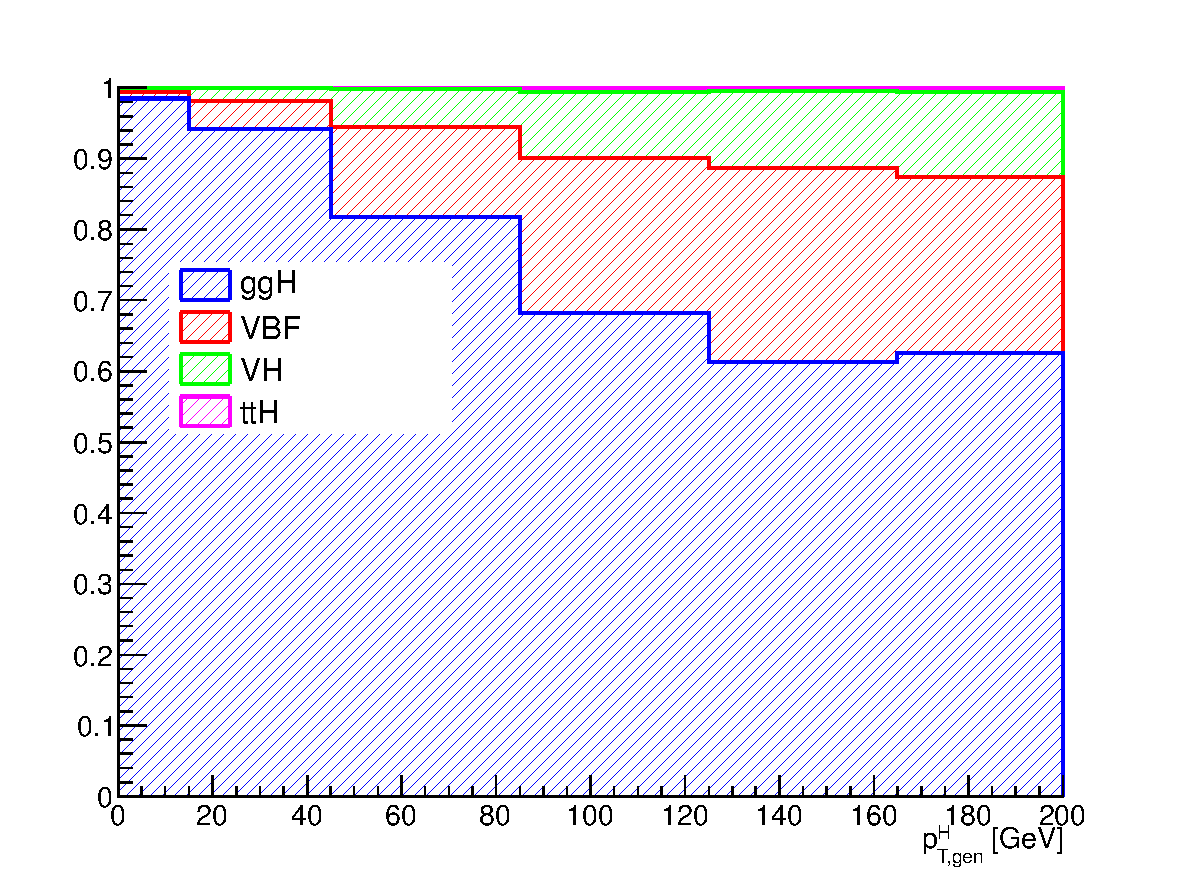
\includegraphics[width=0.7\textwidth]{images/signal_composition_ttH.pdf}
\caption{Relatve fraction of ggH, VBF, VH and ttH in each bin of the Higgs boson transverse momentum.}\label{fig:signal_comp}
\end{figure}
